\documentclass{beamer}
%\usetheme{CambridgeUS}
\usefonttheme{professionalfonts}
\usepackage{times}
\usepackage{tikz}
\usepackage{amsmath}
\usepackage{verbatim}
\usepackage{graphicx}
\usepackage{hyperref}
\usetikzlibrary{arrows,shapes}

\mode<presentation>
{
  \usetheme{Frankfurt}      % or try Darmstadt, Madrid, Warsaw, ...
  \usecolortheme{crane} % or try albatross, beaver, crane, ...
  \usefonttheme{default}  % or try serif, structurebold, ...
  \setbeamertemplate{navigation symbols}{}
  \setbeamertemplate{caption}[numbered]
}

\author{Students of ISU}
\title{Implementing Euler's numerical method in Python}

\begin{document}

\begin{frame}
  \titlepage
\end{frame}

\begin{frame}{Stated problem}

  \begin{block}{Given: Differential Equation}
    \begin{align}
      f(t,T(t)) & = \frac{dT}{dt}=-k(T(t)-T_{env}); \\
      \label{du}
      t_0 & = 0, \quad T(t_0)=T_0.
    \end{align}
  \end{block}

  \begin{block}{Find:}
    \[
      T(t),\quad t>=t_0.
    \]
  \end{block}
\end{frame}
\begin{frame}{Euler's method of numerical integration}
  \begin{align*}
    \Delta x & = h = 0.001\;\; s,\\
    t_i & = t_0 + n\cdot h, \\
    dT(t) & = f(t,T(t))\cdot dt.\\
    \Delta T (t_{i+1}) & = f(t_i,T(t_i))\cdot h,\\
    T(0) & =T_{env},\quad t_0=0.
  \end{align*}
\end{frame}

\begin{frame}
  \frametitle{Program outline}
  TODO: Add program outline with comments
\end{frame}

\begin{frame}{Result of the modeling}
  \begin{center}
  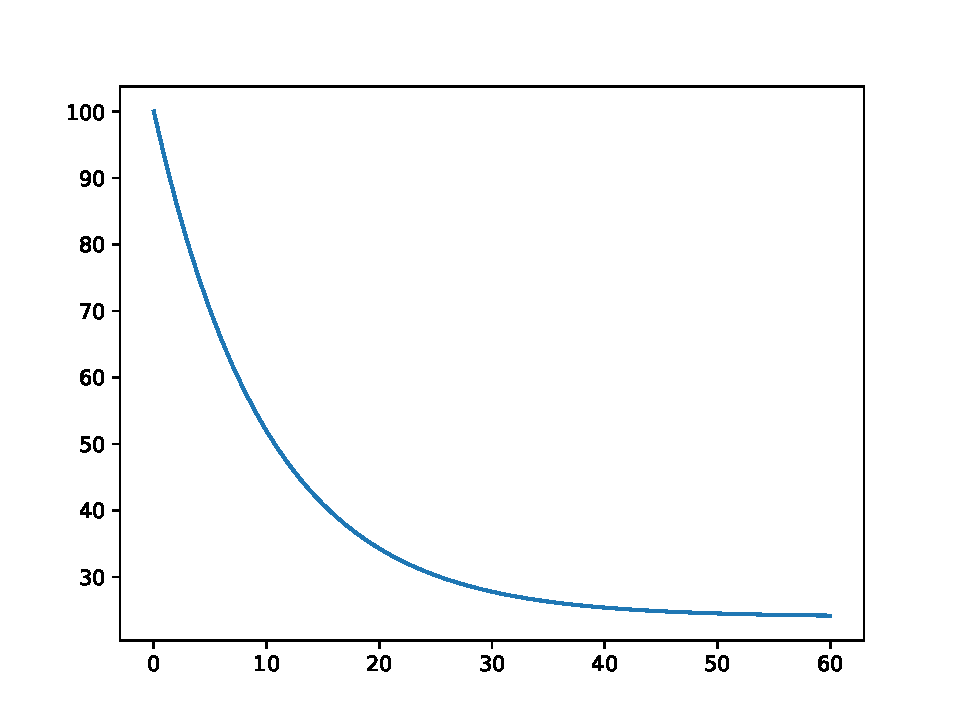
\includegraphics[width=0.8\linewidth]{trajectory.pdf}
\end{center}
\end{frame}
\begin{frame}{Conclusion}

  We have implemented a program realizing Euler's method of numerical solution of the kettle problem\ldots\\[2em]
  Further directions see at the following address:\\
  \url{http://edu.irnok.net/doku.php?id=euler:start}
\end{frame}


\end{document}







%%% Local Variables:
%%% mode: latex
%%% TeX-master: t
%%% End:
